% Shared style for all Git & GitHub lectures (same look as the N-body course)
\documentclass[11pt,a4paper]{article}
\usepackage[margin=2.3cm]{geometry}
\usepackage[T1]{fontenc}
\usepackage{lmodern}
\usepackage{upquote}   % straight quotes in monospaced text, so commands can be copied
\usepackage{microtype}
% keep '--' as two real hyphens in monospace text (commands like --version)
\DisableLigatures[-,<,>]{family=tt*}
\usepackage{booktabs,enumitem,graphicx,xcolor}
\usepackage{array}
\usepackage{needspace}
\usepackage{longtable}
\usepackage{float}
\usepackage{tikz}
\usetikzlibrary{arrows.meta,calc,positioning,decorations.pathreplacing,shapes.geometric,fit,backgrounds}
\usepackage[most]{tcolorbox}
\usepackage{listings}
\usepackage{fancyhdr}
\usepackage[colorlinks=true,linkcolor=blue!50!black,urlcolor=blue!50!black,citecolor=blue!50!black]{hyperref}

\setlength{\parindent}{0pt}
\setlength{\parskip}{0.6em}
\setlength{\abovecaptionskip}{4pt}
\usepackage[font=small,labelfont=bf]{caption}
\setlist{itemsep=0.2em,topsep=0.3em}

% ---------- colours ----------
\definecolor{cbg}{HTML}{F6F8FA}
\definecolor{ckw}{HTML}{0B5CAD}
\definecolor{ccm}{HTML}{6A737D}
\definecolor{cst}{HTML}{B5451B}
\definecolor{cpart}{HTML}{1F6FB2}
\definecolor{cheavy}{HTML}{C0392B}
\definecolor{cgreen}{HTML}{2E8B57}

% ---------- terminal listings ----------
% In a terminal session, lines starting with "$" are what YOU type.
% Everything else is what Git prints back.
\lstdefinestyle{term}{
  basicstyle=\ttfamily\small, backgroundcolor=\color{cbg},
  frame=single, rulecolor=\color{black!15}, showstringspaces=false,
  breaklines=true, columns=fullflexible, keepspaces=true,
  aboveskip=0.6em, belowskip=0.6em, xleftmargin=4pt, xrightmargin=4pt,
  literate={\$\ }{{\textcolor{cgreen}{\$\ }}}2,
  upquote=true
}
\lstset{style=term}
\newcommand{\code}[1]{\texttt{\small #1}}

% ---------- boxes ----------
\newtcolorbox{history}{colback=yellow!8,colframe=orange!60!black,
  title={History},fonttitle=\bfseries\small,left=4pt,right=4pt,top=2pt,bottom=2pt}
\newtcolorbox{quickfact}{colback=purple!4,colframe=purple!55!black,
  title={Quick fact},fonttitle=\bfseries\small,left=4pt,right=4pt,top=2pt,bottom=2pt}
\newtcolorbox{keyidea}{colback=blue!4,colframe=blue!50!black,
  title={Key idea},fonttitle=\bfseries\small,left=4pt,right=4pt,top=2pt,bottom=2pt}
\newtcolorbox{pitfall}{colback=red!4,colframe=red!55!black,
  title={Pitfall},fonttitle=\bfseries\small,left=4pt,right=4pt,top=2pt,bottom=2pt}
\newtcolorbox{tryit}{colback=teal!5,colframe=teal!55!black,
  title={Try it},fonttitle=\bfseries\small,left=4pt,right=4pt,top=2pt,bottom=2pt,breakable}
\newtcolorbox{homework}[1]{colback=green!4,colframe=green!40!black,
  title={Homework #1},fonttitle=\bfseries\small,left=4pt,right=4pt,top=2pt,bottom=2pt,
  breakable}
\newtcolorbox{goals}{colback=gray!6,colframe=gray!60!black,
  title={Learning goals},fonttitle=\bfseries\small,left=4pt,right=4pt,top=2pt,bottom=2pt}

% Solutions always start on a fresh page, behind a clear warning.
\newcommand{\solutionspage}{%
  \clearpage
  \begin{tcolorbox}[colback=red!6,colframe=red!60!black,halign=center]
    {\Large\bfseries Solutions}\\[0.3em]
    {\small Stop here if you have not tried the homework yet.\\
    Attempt every task first, run the checker, and only then read on.}
  \end{tcolorbox}
}

% ---------- Git diagram styles (TikZ) ----------
\tikzset{
  commit/.style={circle,draw=black!70,fill=blue!10,minimum size=7mm,inner sep=0pt,font=\scriptsize\ttfamily},
  newcommit/.style={commit,fill=orange!25,dashed},
  tag/.style={draw,rounded corners=2pt,font=\scriptsize\ttfamily,inner sep=2pt},
  branchtag/.style={tag,fill=green!15,draw=green!40!black},
  headtag/.style={tag,fill=yellow!30,draw=orange!70!black},
  remotetag/.style={tag,fill=purple!10,draw=purple!60!black},
  area/.style={draw,rounded corners,minimum height=11mm,minimum width=33mm,align=center,font=\small},
  cmdarrow/.style={->,thick,>=Stealth},
  link/.style={->,thick,>=Stealth,black!70},
}

% ---------- header ----------
\pagestyle{fancy}
\fancyhf{}
\renewcommand{\headrulewidth}{0.3pt}
\fancyfoot[C]{\thepage}
\newcommand{\lecturetitle}[3]{%
  \fancyhead[L]{\small\textit{Git \& GitHub from Zero}}
  \fancyhead[R]{\small Lecture #1}
  \begin{center}
    {\Large\bfseries Lecture #1}\\[0.4em]
    {\LARGE\bfseries #2}\\[0.4em]
    {\small #3}
  \end{center}
  \vspace{0.5em}
}

\tikzset{
  cbx/.style={draw,rounded corners,fill=blue!6,minimum width=1.9cm,minimum height=8mm,align=center,font=\scriptsize\ttfamily,inner sep=2pt}}
\begin{document}
\lecturetitle{7}{Pull Requests, Forks, and Code Review}{Proposing a change, discussing it, merging it, and working on other people's projects}

\begin{goals}
\begin{itemize}
  \item Explain what a pull request is and walk through its life from branch to merge.
  \item Open a pull request, and review one: comments, suggestions, approve, request changes.
  \item Choose between GitHub's three merge buttons.
  \item Contribute to a project you do not own: fork, clone, \code{upstream}, and keeping your fork in sync.
  \item Inspect and test a teammate's branch on your own computer.
\end{itemize}
\end{goals}

\section{What is a pull request?}

In Lecture 5 you merged a branch yourself, with one command. On a team, you usually should \emph{not} do that unilaterally: someone else should look at the change first. A \textbf{pull request} (PR) is a \emph{request to merge a branch}, shown as a web page where people can read the changes, discuss them, and finally merge them.

\begin{keyidea}
A pull request is a GitHub feature, not a Git command. Git only knows branches and merges. GitHub adds the page around a branch: the list of changes, the conversation, the approvals, and a button to merge. The name comes from the project's \emph{maintainer} (the person who looks after it) \emph{pulling} your work into their repository.
\end{keyidea}

The whole life of a change on a team looks like this:

\begin{figure}[H]
\centering
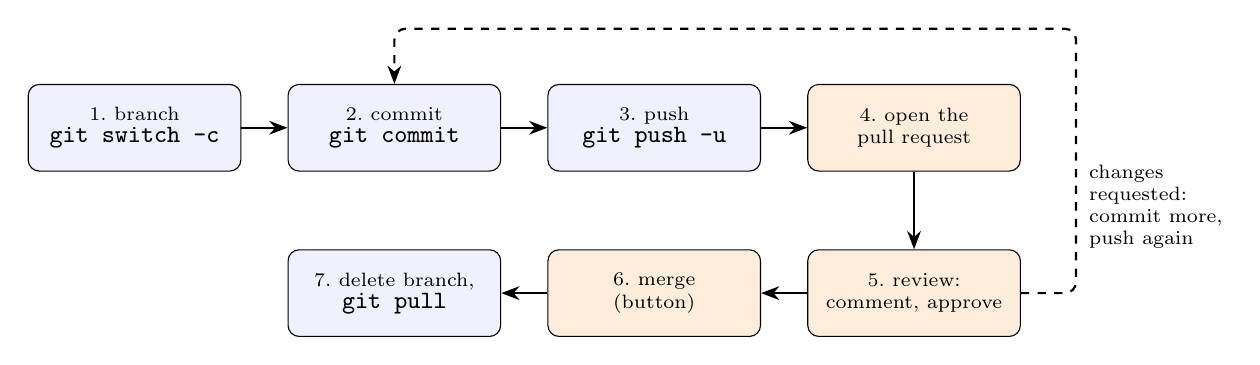
\begin{tikzpicture}[
  blk/.style={draw,rounded corners,fill=blue!6,minimum width=2.7cm,minimum height=11mm,align=center,font=\scriptsize,inner sep=3pt},
  hum/.style={blk,fill=orange!14},
  arr/.style={->,thick,>=Stealth}]
  \node[blk] (b1) at (0,0) {1.\ branch\\\code{git switch -c}};
  \node[blk] (b2) at (3.3,0) {2.\ commit\\\code{git commit}};
  \node[blk] (b3) at (6.6,0) {3.\ push\\\code{git push -u}};
  \node[hum] (b4) at (9.9,0) {4.\ open the\\pull request};
  \node[hum] (b5) at (9.9,-2.1) {5.\ review:\\comment, approve};
  \node[hum] (b6) at (6.6,-2.1) {6.\ merge\\(button)};
  \node[blk] (b7) at (3.3,-2.1) {7.\ delete branch,\\\code{git pull}};
  \draw[arr] (b1)--(b2); \draw[arr] (b2)--(b3); \draw[arr] (b3)--(b4); \draw[arr] (b4)--(b5);
  \draw[arr] (b5)--(b6); \draw[arr] (b6)--(b7);
  \draw[arr,dashed,rounded corners] (b5.east) -- ++(0.7,0) |- ($(b2.north)+(0,0.7)$) -- (b2.north);
  \node[font=\scriptsize,anchor=west,align=left] at (12.0,-1.0) {changes\\requested:\\commit more,\\push again};
\end{tikzpicture}
\caption{The pull-request workflow. Orange steps happen on the website; blue steps are the Git commands you already know. If the reviewer asks for changes (dashed), you commit more on the same branch and push; the pull request updates by itself.}
\label{fig:prflow}
\end{figure}

\section{Opening a pull request}

Suppose you work in a repository you may push to: your own, or a team's where you are a \emph{collaborator} (someone the owner invited under Settings $\rightarrow$ Collaborators; the invitation must be accepted). Everyone else cannot push, and uses a \emph{fork} instead (Section~\ref{sec:forks}). Create a branch, commit, and push it, exactly as in Lecture 6:

\Needspace{8\baselineskip}
\begin{lstlisting}
$ git switch -c add-note
$ echo "Remember to drink water." > note.md
$ git add note.md
$ git commit -m "Add a hydration note"
$ git push -u origin add-note
\end{lstlisting}

Now open the repository on github.com. Right after the push a yellow banner appears with a button \textbf{Compare \& pull request} (otherwise: \textbf{Pull requests $\rightarrow$ New pull request}). The form asks:

\begin{itemize}
  \item \textbf{base} (the branch you want to merge \emph{into}, usually \code{main}) and \textbf{compare} (your branch; GitHub also calls it the \emph{head}). Check them: ``merge \code{add-note} into \code{main}''.
  \item A \textbf{title}, in the style of a commit message: short and imperative.
  \item A \textbf{description}: \emph{what} you changed and \emph{why}, and anything the reviewer should look at. (Use \code{Closes \#12} to link an issue; Lecture 9.)
\end{itemize}

Press \textbf{Create pull request}. You get a page with the conversation, the list of commits, and a \textbf{Files changed} tab. That tab is the same comparison as \code{git diff main...add-note} on your computer.

\begin{quickfact}
The three dots in \code{git diff main...add-note} mean ``the changes on \code{add-note} since it split off from \code{main}'': your work, without whatever else happened on \code{main} meanwhile. (For \code{git log}, \code{main..add-note} with two dots means ``the commits on \code{add-note} that \code{main} lacks''.)
\end{quickfact}

\begin{quickfact}
A good pull request is \emph{small} (one idea, a few files) with a clear title and description. Reviewers read small requests carefully and big ones badly. If your work is not ready, choose \textbf{Create draft pull request}: it cannot be merged until you press \textbf{Ready for review}.
\end{quickfact}

\section{Reviewing a pull request}

A \textbf{review} is a colleague reading your change before it joins \code{main}. Reasons: catching mistakes, sharing knowledge, keeping the code consistent. Nobody is perfect, and fresh eyes find typos you cannot see.

As a reviewer, open the \textbf{Files changed} tab:

\begin{itemize}
  \item Hover over a line number and click the blue \textbf{+} to add an \emph{inline comment} on that line.
  \item Instead of describing a fix, you can \textbf{suggest} it: the \emph{Add a suggestion} button in the comment box inserts a block with the corrected text. The author can accept it with one click.
  \item When you have read everything, press \textbf{Review changes}, choose one of three verdicts, and \textbf{Submit review}:
\end{itemize}

\begin{center}
\small
\begin{tabular}{@{}l >{\raggedright\arraybackslash}p{9.4cm}@{}}
\toprule
Verdict & Meaning \\
\midrule
\textbf{Comment} & General feedback, no decision. \\
\textbf{Approve} & ``This is good to merge.'' \\
\textbf{Request changes} & ``Please fix the points I raised first.'' \\
\bottomrule
\end{tabular}
\end{center}

You cannot approve your own pull request, which is why review needs two people. As the author, you answer in the conversation (a reviewer's suggestion is applied with \textbf{Commit suggestion}) and \emph{fix by committing}: make the change on your branch and push it. You do not open a new request; the same pull request picks up the new commits. When a comment is dealt with, mark the conversation as resolved.

\begin{keyidea}
Review the \emph{code}, never the person. Be specific (``this variable name is confusing: maybe \code{total\_price}?''), explain why, say what is good too, and ask questions rather than issue orders. When you receive a review, remember that every comment is about the change, not about you.
\end{keyidea}

\section{Keeping your pull request mergeable}

\textbf{Conflicts.} If someone merged other changes meanwhile, GitHub may say \emph{This branch has conflicts that must be resolved}. Solve it on your computer: merge \code{main} into your branch, resolve the conflict (Lecture 5), commit and push; the pull request updates.

\begin{lstlisting}
$ git switch add-note
$ git fetch origin
$ git merge origin/main        # fix the conflict if there is one, then commit
$ git push
\end{lstlisting}

\begin{pitfall}
Do not start your branch from an old \code{main}. Before a new branch, run \code{git switch main}, \code{git pull}, and only then \code{git switch -c new-branch}. Otherwise you carry old code and invite conflicts.
\end{pitfall}

\section{Merging: three buttons}

When the review is positive, the green merge button offers three ways to merge:

\begin{figure}[H]
\centering
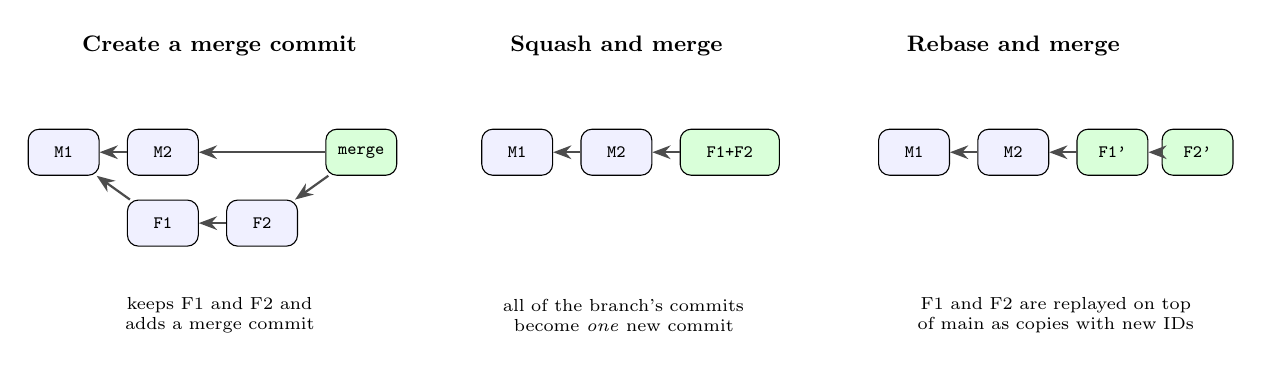
\begin{tikzpicture}[scale=0.9,transform shape,
  cbx/.style={draw,rounded corners,fill=blue!6,minimum width=1.0cm,minimum height=6.5mm,align=center,font=\scriptsize\ttfamily,inner sep=1pt},
  new/.style={cbx,fill=green!15},
  ttl/.style={font=\small\bfseries,align=center},
  bcap/.style={font=\scriptsize,align=center,text width=4.6cm}]
  % (a) merge commit
  \node[ttl] at (2.2,1.5) {Create a merge commit};
  \node[cbx] (a1) at (0,0) {M1}; \node[cbx] (a2) at (1.4,0) {M2};
  \node[cbx] (af1) at (1.4,-1.0) {F1}; \node[cbx] (af2) at (2.8,-1.0) {F2};
  \node[new] (ax) at (4.2,0) {merge};
  \draw[link] (a2)--(a1); \draw[link] (af1)--(a1); \draw[link] (af2)--(af1);
  \draw[link] (ax)--(a2); \draw[link] (ax)--(af2);
  % (b) squash
  \node[ttl] at (7.8,1.5) {Squash and merge};
  \node[cbx] (b1) at (6.4,0) {M1}; \node[cbx] (b2) at (7.8,0) {M2};
  \node[new,minimum width=1.4cm] (bs) at (9.4,0) {F1+F2};
  \draw[link] (b2)--(b1); \draw[link] (bs)--(b2);
  % (c) rebase
  \node[ttl] at (13.4,1.5) {Rebase and merge};
  \node[cbx] (c1) at (12.0,0) {M1}; \node[cbx] (c2) at (13.4,0) {M2};
  \node[new] (cr1) at (14.8,0) {F1'}; \node[new] (cr2) at (16.0,0) {F2'};
  \draw[link] (c2)--(c1); \draw[link] (cr1)--(c2); \draw[link] (cr2)--(cr1);
  \node[bcap] at (2.2,-2.3) {keeps F1 and F2 and adds a merge commit};
  \node[bcap] at (7.9,-2.3) {all of the branch's commits become \emph{one} new commit};
  \node[bcap] at (14.0,-2.3) {F1 and F2 are replayed on top of main as copies with new IDs};
\end{tikzpicture}
\caption{The three merge buttons. \code{M1}, \code{M2} are on \code{main}; \code{F1}, \code{F2} are the commits of the pull request's branch. Green commits are new.}
\label{fig:buttons}
\end{figure}

\begin{description}[leftmargin=1.2em,style=nextline]
\item[Create a merge commit] The merge you know from Lecture 5. Keeps every commit and the real history. A safe default.
\item[Squash and merge] Combines all commits of the branch into one. Good when the branch has messy ``fix typo'' commits and you want a tidy \code{main}. The branch's own commits are not kept in \code{main}.
\item[Rebase and merge] Replays the commits on top of \code{main} without a merge commit, giving a straight line. Lecture 8 explains rebasing; for now just know it exists.
\end{description}

After merging, press \textbf{Delete branch}: it has done its job (Lecture 5's life cycle). Then bring the result to your computer and tidy up:

\begin{lstlisting}
$ git switch main
$ git pull
$ git branch -d add-note        # fine after a merge commit
\end{lstlisting}

(After \emph{Squash and merge} or \emph{Rebase and merge}, GitHub created \emph{new} commits, so Git cannot see that your branch's commits are included. Depending on whether Git still has the old \code{origin/add-note} label, \code{-d} then either refuses (``not fully merged'') or succeeds with a warning. If it refuses and you checked on GitHub that the pull request is merged, use \code{git branch -D add-note}. This is one of the rare safe uses of \code{-D}: you checked on GitHub that the pull request was merged.)

\section{Looking at a teammate's branch}\label{sec:teammate}

\textbf{Looking at a teammate's branch before you review it.} Fetch, look, and (if you want to run it) check it out:

\Needspace{12\baselineskip}
\begin{lstlisting}
$ git fetch
$ git log --oneline main..origin/teammate-feature     # commits it adds
6bce7d7 Document greeting
14ff5f7 Add greeting
$ git diff --stat main...origin/teammate-feature     # files it changes
 README.md    | 1 +
 greeting.txt | 1 +
 2 files changed, 2 insertions(+)
$ git switch teammate-feature
branch 'teammate-feature' set up to track 'origin/teammate-feature'.
\end{lstlisting}

\code{git switch} on a name that exists only on the remote creates a local branch that tracks it. If you have write access you may push a fix to that same branch; the open pull request then shows it.

\section{Forks: contributing to a project you do not own}\label{sec:forks}

You cannot push to someone else's repository (nor should you be able to). Open-source projects therefore use \textbf{forks}. A fork is your own copy of the repository, \emph{on GitHub, under your account}. You push to your fork, and then ask the owner to pull from it.

\begin{figure}[H]
\centering
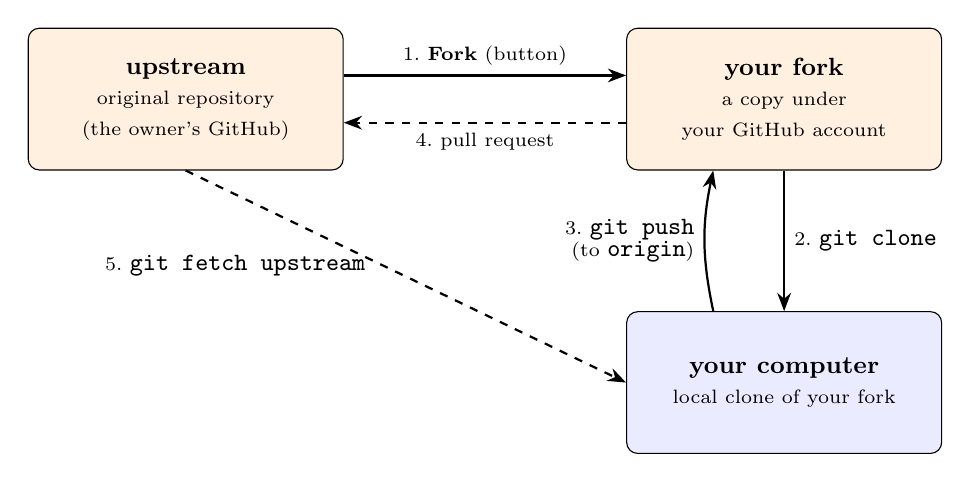
\begin{tikzpicture}[
  box/.style={draw,rounded corners,minimum width=4.0cm,minimum height=1.8cm,align=center,font=\small},
  arr/.style={->,thick,>=Stealth}]
  \node[box,fill=orange!12] (up) at (0,3.6) {\textbf{upstream}\\\scriptsize original repository\\\scriptsize (the owner's GitHub)};
  \node[box,fill=orange!12] (fk) at (7.6,3.6) {\textbf{your fork}\\\scriptsize a copy under\\\scriptsize your GitHub account};
  \node[box,fill=blue!8] (lo) at (7.6,0) {\textbf{your computer}\\\scriptsize local clone of your fork};
  \draw[arr] ([yshift=3mm]up.east) -- node[above,font=\scriptsize] {1.\ \textbf{Fork} (button)} ([yshift=3mm]fk.west);
  \draw[arr] (fk) -- node[right,font=\scriptsize] {2.\ \code{git clone}} (lo);
  \draw[arr,bend left=12] ([xshift=-0.9cm]lo.north) to node[left,font=\scriptsize,align=right] {3.\ \code{git push}\\(to \code{origin})} ([xshift=-0.9cm]fk.south);
  \draw[arr,dashed] ([yshift=-3mm]fk.west) -- node[below,font=\scriptsize] {4.\ pull request} ([yshift=-3mm]up.east);
  \draw[arr,dashed] (up.south) -- node[pos=0.45,left=3pt,font=\scriptsize,align=right] {5.\ \code{git fetch upstream}} ($(lo.west)+(0,0.0)$);
\end{tikzpicture}
\caption{Three copies. You clone your fork (\code{origin}) and also add the original as a second remote called \code{upstream}, to follow its progress.}
\label{fig:fork}
\end{figure}

\begin{enumerate}
  \item On the original repository's page click \textbf{Fork}, then \textbf{Create fork}.
  \item Clone \emph{your fork} (not the original) and tell Git about the original:
\end{enumerate}

\begin{lstlisting}
$ git clone git@github.com:YOU/project.git
$ cd project
$ git remote add upstream git@github.com:OWNER/project.git
$ git remote -v
origin    git@github.com:YOU/project.git (fetch)
origin    git@github.com:YOU/project.git (push)
upstream  git@github.com:OWNER/project.git (fetch)
upstream  git@github.com:OWNER/project.git (push)
\end{lstlisting}

\code{origin} is your fork, where you may push. \code{upstream} is the original, the usual name for it, where you only \emph{read}. (Do not confuse this remote \emph{name} with the ``upstream branch'' that \code{-u} set up in Lecture 6.) Work as before: a branch per change, push it to \code{origin}, and open the pull request. On the pull-request page, the \emph{base repository} is the owner's, and the \emph{head repository} is your fork.

\subsection{Keeping your fork up to date}

The original keeps moving. To catch up, fetch from \code{upstream} and merge into your \code{main}:

\begin{lstlisting}
$ git fetch upstream
$ git switch main
$ git merge upstream/main          # usually a fast-forward
$ git push origin main             # update your fork on GitHub
\end{lstlisting}

\begin{keyidea}
Never commit your own work directly on the fork's \code{main}; make a branch. Then \code{main} stays a clean mirror of \code{upstream/main}, and catching up is always a simple fast-forward. (GitHub also offers a \textbf{Sync fork} button on your fork's page, which does the same thing on the website.)
\end{keyidea}

\Needspace{12\baselineskip}
\section{Homework 7}

\begin{homework}{7: Review and merge}
\textbf{Part A: be the reviewer and the maintainer} (no internet needed). The setup script creates \code{practice/hw7\_server.git}, a bare repository playing the role of GitHub. A teammate has pushed a branch \code{teammate-feature} and wants it merged into \code{main}. From the course folder:
\begin{lstlisting}
$ bash codeHints/L07/setup_hw7.sh
$ cd practice
\end{lstlisting}
Do the tasks in order. To start over: \code{setup\_hw7.sh --reset} from the course folder.

\begin{description}[leftmargin=1.2em,style=nextline]
\item[7.1 Clone] Clone the server into a folder called \code{hw7} and go into it.
\item[7.2 Review] Run \code{git fetch}, then look at the commits the branch adds and at its changes, using the commands of Section~\ref{sec:teammate}. One line contains a typo. In \code{practice/hw7\_answers.txt} (next to the \code{hw7} folder, created with \code{printf} or \code{echo}) write two lines: \code{commits=<number of commits on the branch>} and \code{typo-in=<file name containing the typo>}.
\item[7.3 Suggest a fix] Check out the branch (\code{git switch teammate-feature}), fix the typo, commit it as \code{Fix typo in greeting}, and push to the same branch with \code{git push}.
\item[7.4 Merge] Switch to \code{main} and merge the branch \emph{with a merge commit}: \code{git merge --no-ff --no-edit teammate-feature}. Push \code{main}.
\item[7.5 Clean up] Delete the branch locally (\code{git branch -d}) and on the server (\code{git push origin --delete teammate-feature}).
\item[7.6 Question] On GitHub, which of the three merge buttons would produce the same result as your command in 7.4 (all commits kept, plus a merge commit)? Add the line \code{merge-button=<word>} with \code{merge}, \code{squash} or \code{rebase}.
\end{description}

\textbf{Part B: real pull requests with your friend} (optional, but this is the point of the lecture). You need two GitHub accounts, called \textbf{A} and \textbf{B}. Before you start: both repositories must be created as \textbf{Public} (not Private), because the checker looks them up without logging in; and if you ticked ``Block command line pushes that expose my email'' in Lecture 6, make sure \code{git config user.email} in your clone is your no-reply address. The two rounds are done one after the other. \emph{Each of you ends up with exactly one clone, \code{practice/hw7\_pr}}: B's from Round 1, A's from Round 2 (it is not the same as \code{practice/hw7} of Part A). Run the clone commands from the course folder.

\begin{description}[leftmargin=1.2em,style=nextline]
\item[7.7 Round 1: shared repository, B's pull request] \textbf{A} creates a \emph{Public} repository \code{pr-practice} with a README (ticking ``Add a README'' is fine here), and adds \textbf{B} under Settings $\rightarrow$ Collaborators $\rightarrow$ Add people (type B's exact user name). \textbf{B} \emph{must accept the invitation}: open the e-mail from GitHub, or go to \code{github.com/A/pr-practice/invitations}. Until B accepts, a push fails with ``Permission denied'' or ``403''. Then \textbf{B} clones into \code{practice/hw7\_pr}, creates the branch \code{add-b-note} with a new file \code{notes-from-b.md}, pushes it, and opens a pull request with a title and a description. \textbf{A} reviews: at least one inline comment (use \emph{Add a suggestion} once), then \emph{Submit review} with \emph{Request changes}. \textbf{B} responds (clicking \emph{Commit suggestion}, or committing a fix on the same branch and pushing). \textbf{A} approves and merges with \emph{Create a merge commit}. \textbf{B} presses \emph{Delete branch}, then in the clone: \code{git switch main}, \code{git pull}, \code{git branch -d add-b-note}.
\item[7.8 Round 2: fork, A's pull request] Swap roles. \textbf{B} creates a \emph{Public} repository \code{pr-practice-b} with a README. \textbf{A} forks it and clones \emph{the fork} into \code{practice/hw7\_pr}, runs \code{git remote add upstream} with B's repository address, creates the branch \code{add-a-note} with a new file, pushes it to the fork, and opens a pull request \emph{to B's repository} (check that the base repository is B's). \textbf{B} reviews with a suggestion and requests changes. \textbf{A} clicks \emph{Commit suggestion}. \textbf{B} approves and merges with \emph{Squash and merge}. \textbf{A} syncs the fork: \code{git fetch upstream}, \code{git switch main}, \code{git merge upstream/main}, \code{git push origin main}. (A's local \code{add-a-note} may be behind GitHub's copy now; harmless, since A only syncs \code{main}.)
\item[7.9 Record and check] Each of you records the pull request \emph{you opened}: \textbf{B} the one from Round 1, \textbf{A} the one from Round 2. In \code{practice/hw7\_pr\_answers.txt} write one line \code{my-pr=<owner>/<repository>\#<number>}, for example \code{my-pr=alice/pr-practice\#1}. Read the number from the top of the pull request page (a second attempt may be \code{\#2}). Be on \code{main} with a clean working directory, and run the checker.
\end{description}

\textbf{Check yourself:} \code{bash codeHints/L07/check\_hw7.sh} from the course folder. Part A needs no network. Part B is checked only if \code{practice/hw7\_pr} or \code{hw7\_pr\_answers.txt} exists; the checker asks GitHub's public service whether your pull request is merged, and skips that one check if it cannot reach GitHub. Then compare with the solutions at the end of this lecture.
\end{homework}

\section{Summary}

\begin{itemize}
  \item A pull request is a reviewable proposal to merge a branch. Branch, commit, push, open, review, merge, delete, pull.
  \item Reviewers comment, suggest, approve or request changes; authors answer by pushing more commits to the same branch.
  \item Merge with a merge commit (keeps everything), squash (one commit) or rebase (straight line); then delete the branch.
  \item Fork what you cannot push to: clone the fork as \code{origin}, add the original as \code{upstream}, branch for each change, merge \code{upstream/main} to stay current.
\end{itemize}

\textbf{Further reading:} \emph{Pro Git}, Chapter 6.2; GitHub Docs, ``About pull requests''.

\solutionspage

\section*{Solutions to Homework 7}

\textbf{Part A.}

\begin{lstlisting}
$ bash codeHints/L07/setup_hw7.sh
$ cd practice
$ git clone hw7_server.git hw7
$ cd hw7
$ git fetch
$ git log --oneline main..origin/teammate-feature     # 2 commits
$ git diff main...origin/teammate-feature             # "Helo, world" in greeting.txt
$ printf 'commits=2\ntypo-in=greeting.txt\nmerge-button=merge\n' > ../hw7_answers.txt
$ git switch teammate-feature
$ sed -i.bak 's/Helo/Hello/' greeting.txt && rm greeting.txt.bak    # or edit by hand
$ git commit -am "Fix typo in greeting"
$ git push
$ git switch main
$ git merge --no-ff --no-edit teammate-feature
$ git push
$ git branch -d teammate-feature
$ git push origin --delete teammate-feature
\end{lstlisting}

\textbf{7.2.} The branch adds two commits (\code{Add greeting} and \code{Document greeting}). The typo is \code{Helo} in \code{greeting.txt}. (\code{git diff} with three dots shows only what the branch added.)

\textbf{7.3.} \code{git switch teammate-feature} finds no local branch of that name, but there is \code{origin/teammate-feature}, so Git creates a tracking branch for you. A plain \code{git push} then updates the remote branch, as when you push a fix to an open pull request.

\textbf{7.4.} \code{--no-ff} forces a merge commit even though a fast-forward would be possible. This is what GitHub's button \emph{Create a merge commit} does, hence the answer \code{merge}. (The checker expects a merge commit at the tip of the server's \code{main}; a fast-forward would fail.)

\textbf{7.5.} \code{git branch -d} works because the branch is merged. \code{git push origin --delete} removes it on the server (on GitHub, the \emph{Delete branch} button).

\textbf{Part B.} Replace \code{A}, \code{B} by your account names.

\textbf{Round 1: shared repository (B opens the pull request).}

{\small
\begin{longtable}{@{}c p{0.84\textwidth}@{}}
\toprule
Who & Step \\
\midrule
\endhead
A & Create a \emph{public} repository \code{pr-practice} with a README. Settings $\rightarrow$ Collaborators $\rightarrow$ Add people: B. \\
B & Accept the invitation (e-mail, or \code{github.com/A/pr-practice/invitations}). \\
B & \code{git clone git@github.com:A/pr-practice.git practice/hw7\_pr}, then \code{cd practice/hw7\_pr}. \\
B & \code{git switch -c add-b-note}, create \code{notes-from-b.md}, \code{git add}, \code{git commit}, \code{git push -u origin add-b-note}. \\
B & On GitHub: \emph{Compare \& pull request}, title and description, \emph{Create pull request}. \\
A & \emph{Files changed}: inline comment with a suggestion; \emph{Review changes} $\rightarrow$ \emph{Request changes} $\rightarrow$ \emph{Submit review}. \\
B & \emph{Commit suggestion} (or fix locally: \code{git commit}, \code{git push}). \\
A & \emph{Approve}; \emph{Create a merge commit}; confirm. \\
B & \emph{Delete branch}; locally \code{git switch main}, \code{git pull}, \code{git branch -d add-b-note}. \\
B & \code{printf 'my-pr=A/pr-practice\#1\textbackslash n' > ../hw7\_pr\_answers.txt} (from inside \code{hw7\_pr}). \\
\bottomrule
\end{longtable}}

\textbf{Round 2: fork (A opens the pull request).}

{\small
\begin{longtable}{@{}c p{0.84\textwidth}@{}}
\toprule
Who & Step \\
\midrule
\endhead
B & Create a \emph{public} repository \code{pr-practice-b} with a README. \\
A & \emph{Fork} the repository, then \code{git clone git@github.com:A/pr-practice-b.git practice/hw7\_pr}. \\
A & \code{git remote add upstream git@github.com:B/pr-practice-b.git}; \code{git remote -v} shows both remotes. \\
A & \code{git switch -c add-a-note}, add a file, commit, \code{git push -u origin add-a-note}. \\
A & On GitHub open the pull request; check that the base repository is \code{B/pr-practice-b}. \\
B & Review with a suggestion and \emph{Request changes}. \\
A & \emph{Commit suggestion}. \\
B & \emph{Approve}; \emph{Squash and merge}. \\
A & \code{git fetch upstream}, \code{git switch main}, \code{git merge upstream/main}, \code{git push origin main}. \\
A & \code{printf 'my-pr=B/pr-practice-b\#1\textbackslash n' > ../hw7\_pr\_answers.txt}. \\
\bottomrule
\end{longtable}}

In Round 1, A has no local clone, and in Round 2, B has none; the names and the numbers \code{\#1} above are placeholders. Each of you writes the pull request \emph{you opened}: B the one from Round 1, A the one from Round 2. Both repositories must be public, because the checker asks GitHub's public service whether the pull request is merged. If the line is missing the checker skips nothing silently: a missing or private pull request is reported as a failure, while an unreachable GitHub (no network, or more than 60 anonymous requests an hour) skips only that one check. The \code{upstream} check applies only to the fork route (A). After Round 2, A's \code{practice/hw7\_pr} is the fork clone, so \code{origin} points at A's fork on github.com and \code{upstream} at B's repository.

\Needspace{8\baselineskip}
\textbf{Common mistakes.}
\begin{itemize}
  \item Merging with a fast-forward in 7.4 (\code{git merge teammate-feature} without \code{--no-ff}): the server's \code{main} then has no merge commit and the checker fails 7.4. Reset and redo.
  \item Opening the pull request \emph{to your own fork}. Check that the base repository is the original owner's.
  \item B not accepting the collaborator invitation: the push in Round 1 fails with ``Permission denied''.
  \item Creating a repository as \emph{Private}: the checker reports ``GitHub cannot find ...''.
  \item Forgetting \code{upstream}, then wondering why \code{git fetch upstream} fails (``not a git repository'' or ``no such remote'').
  \item Writing the pull request number of your \emph{partner's} request, or a private repository, in \code{hw7\_pr\_answers.txt}.
  \item \code{git branch -d} refusing after \emph{Squash and merge}: expected (see the lecture); if the pull request really is merged, \code{git branch -D} is fine.
\end{itemize}


\end{document}
